
\chapter[Internal Heat of ...]{Internal Heat of the \\Earth}

\begin{figure}[ht]
    \vspace{-40pt}
    %\begin{adjustwidth}{-0.9cm}{-0cm}
        \fbox{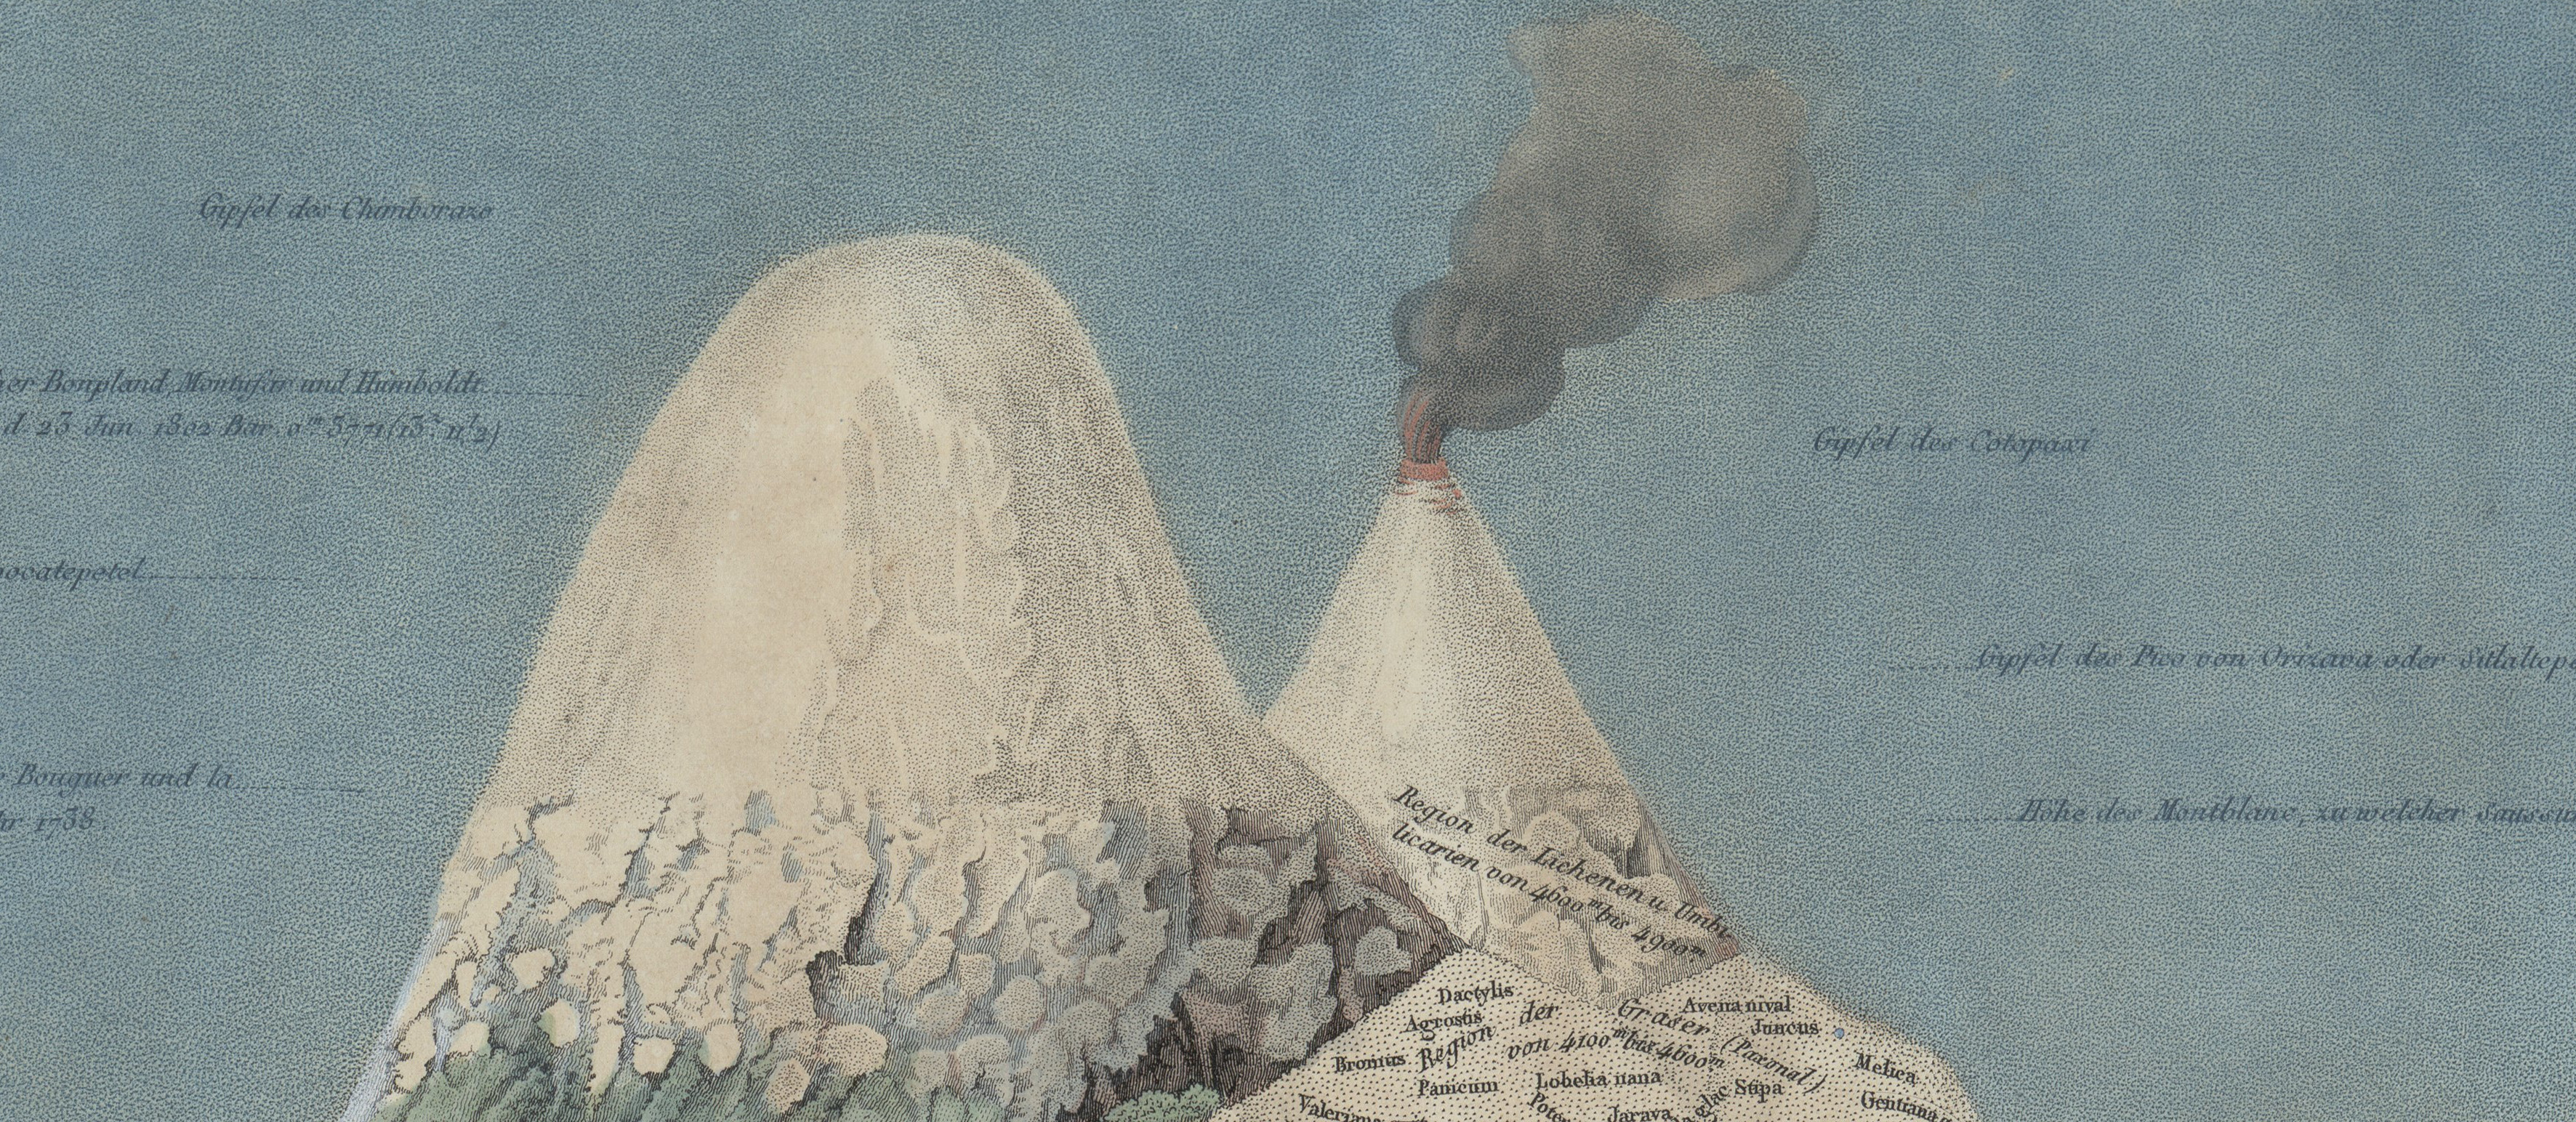
\includegraphics[width=\linewidth,height=.225\paperheight]{../../pictures/tableau-physique-cropped-4.jpg}}
        \caption{\footnotesize Humboldt, \emph{Tableau Physique} (1807). Public domain.}
    %\end{adjustwidth}
\end{figure}

\lettrine[lines=4]{\goudy T}{he} figure of the Earth and the amount of solidification (density) which it has acquired are intimately connected with the forces by which it is animated, in so far, at least, as they have been excited or awakened from without, through its planetary position with reference to a luminous central body. Compression, when considered as a consequence of centrifugal force acting on a rotating mass, explains the earlier condition of fluidity of our planet. During the solidification of this fluid, which is commonly conjectured to have been gaseous and primordially heated to a very high temperature, an enormous quantity of latent heat must have been liberated. If the process of solidification began, as Fourier conjectures, by radiation from the cooling surface exposed to the atmosphere, the particles near the center would have continued fluid and hot. As, after long emanation of heat from the center toward the exterior, a stable condition of the temperature of the Earth would at length be established, it has been assumed that with increasing depth the subterranean heat likewise uninterruptedly increases. The heat of the water which flows from deep borings (Artesian wells), direct experiments regarding the temperature of rocks in mines, but, above all, the volcanic activity of the Earth, shown by the flow of molten masses from open fissures, afford unquestionable evidence of this increase for very considerable depths from the upper strata. According to conclusions based certainly upon mere analogies, this increase is probably much greater toward the center.

That which has been learned by an ingenious analytic calculation, expressly perfected for this class of investigations,\footnote{Here we must notice the admirable analytical labors of Fourier, Biot, Laplace, Poisson, Duhamel, and Lam\'{e}. In his Th\'{e}orie Math\'{e}matique de la Chaleur, 1835, p. 3, 428-430, 436, and 521-524 (see, also, De la Rive's abstract in the Bibliotheque Universelle de Gen\'{e}ve), Poisson has developed an hypothesis totally different from Fourier's view (Th\'{e}orie Analytique de la Chaleur.) He denies the present fluid state of the Earth's center; he believes that in cooling by radiation to the medium surrounding the Earth, the parts which were first solidified sunk, and that by a double descending and ascending current, the great inequality was lessened which would have taken place in a solid body cooling from the surface. It seems more probable to this great geometer that the solidification began in the parts lying nearest to the center. The phenomenon of the increase of heat with the depth does not extend to the whole mass of the Earth, and is merely a consequence of the motion of our planetary system in space, of which some parts are of a very different temperature from others, in consequence of stellar heat (chaleur stellaire). Thus, according to Poisson, the warmth of the water of our Artesian wells is merely that which has penetrated into the Earth from without; and the Earth itself might be regarded as in the same circumstances as a mass of rock conveyed from the equator to the pole in so short a time as not to have entirely cooled. The increase of temperature in such a block would not extend to the central strata. The physical doubts which have reasonably been entertained against this extraordinary cosmical view (which attributes to the regions of space that which probably is more dependent on the first transition of matter condensing from the gaseous fluid into the solid state) will be found collected in Poggendorf's Annalen, bd. xxxix., s. 93-100.} regarding the motion of heat in homogeneous metallic spheroids, must be applied with much caution to the actual character of our planet, considering our present imperfect knowledge of the substances of which the Earth is composed, the difference in the capacity of heat and in the conducting power of different superimposed masses, and the chemical changes experienced by solid and liquid masses from any enormous compression. It is with the greatest difficulty that our powers of comprehension can conceive the boundary line which divides the fluid mass of the interior from the hardened mineral masses of the external surface, or the gradual increase of the solid strata, and the condition of semifluidity of the earthy substances, these being conditions to which known laws of hydraulics can only apply under considerable modifications. The Sun and Moon, which cause the sea to ebb and flow, most probably also affect these subterranean depths. We may suppose that the periodic elevations and depressions of the molten mass under the already solidified strata must have caused inequalities in the vaulted surface from the force of pressure. The amount and action of such oscillations must, however, be small; and if the relative position of the attracting cosmical bodies may here also excite spring tides, it is certainly not to these, but to more powerful internal forces, that we must ascribe the movements that shake the Earth's surface. There are groups of phenomena to whose existence it is necessary to draw attention, in order to indicate the universality of the influence of the attraction of the Sun and Moon on the external and internal conditions of the Earth, however little we may be able to determine the quantity of this influence.

According to tolerably accordant experiments in Artesian wells, it has been shown that the heat increases on an average about 1 for every 545 feet. If this increase can be reduced to arithmetical relations, it will follow, as I have already observed\footnote{See the Introduction. This increase of temperature has been found in the Puits de Grenelle, at Paris, at 583 feet; in the boring at the new saltworks at Minden, almost 536; at Pregny, near Geneva, according to Auguste de la Rive and Marcet, notwithstanding that the mouth of the boring is 1609 feet above the level of the sea, it is also 536 feet. This coincidence between the results of a method first proposed by Arago in the year 1821 (Annuaire du Bureau des Longitudes, 1835, p. 234), for three different mines, of the absolute depths of 1794, 2231, and 725 feet respectively, is remarkable. The two points on the Earth, lying at a small vertical distance from each other, whose annual mean temperatures are most accurately known, are probably at the spot on which the Paris Observatory stands, and the Caves de l'Observatoire beneath it. The mean temperature of the former is 5195, and of the latter 533, the difference being 198 for 92 feet, or 1 for 5177 feet. (Poisson, Th\'{e}orie Math. de la Chaleur, p. 415 and 462.) In the course of the last seventeen years, from causes not yet perfectly understood, but probably not connected with the actual temperature of the caves, the thermometer standing there has risen very nearly 094. Although in Artesian wells there are sometimes slight errors from the lateral permeation of water, these errors are less injurious to the accuracy of conclusions than those resulting from currents of cold air, which are almost always present in mines. The general result of Reich's great work on the temperature of the mines in the Saxony mining districts gives a somewhat slower increase of the terrestrial heat, or 1 to 763 feet. (Reich, Beob. uber die Temperatur des Gesteins in verschiedenen Tiefen, 1834, 8. 134.) Phillips, however, found (Pogg., Annalen, bd. xxxiv., s. 191), in a shaft of the coalmine of Monkwearmouth, near Newcastle, in which, as I have already remarked, excavations are going on at a depth of about 1500 feet below the level of the sea, an increase of 1 to 5906 feet, a result almost identical with that found by Arago in the Puits de Grenelle.}, that a stratum of granite would be in a state of fusion at a depth of nearly twenty-one geographical miles, or between four and five times the elevation of the highest summit of the Himalaya.

We must distinguish in our globe three different modes for the transmission of heat. The first is periodic, and affects the temperature of the terrestrial strata according as the heat penetrates from above downward or from below upward, being influenced by the different positions of the Sun and the seasons of the year. The second is likewise an effect of the Sun, although extremely slow -- a portion of the heat that has penetrated into the equatorial regions moves in the interior of the globe toward the poles, where it escapes into the atmosphere and the remoter regions of space. The third mode of transmission is the slowest of all, and is derived from the secular cooling of the globe, and from the small portion of the primitive heat which is still being disengaged from the surface.
    